\documentclass{beamer}
 
\usepackage[utf8]{inputenc}
\usepackage{amsmath}
\usepackage{geometry}
\usepackage{mhchem} % Package for chemical equation typesetting
\usepackage{siunitx} % Provides the \SI{}{} command for typesetting SI units
\usepackage{parskip}
\usepackage{graphicx} % Required for the inclusion of images
\usepackage{amssymb}
\usepackage{placeins}
\usepackage{cancel}
\usepackage{tikz}
\usepackage{listings}
%\usepackage{fullpage}
\usepackage{booktabs, multicol, multirow}
%

% Lots of macros. Thanks to D.F. Gleich for a bunch of these. 

\graphicspath{{./}{./figs/}}

  \def\clap#1{\hbox to 0pt{\hss#1\hss}}
  \def\mathclap{\mathpalette\mathclapinternal}
  \def\mathclapinternal#1#2{%
    \clap{$\mathsurround=0pt#1{#2}$}}

\usepackage{bm}
\providecommand{\mat}[1]{\bm{#1}}%
\renewcommand{\vec}[1]{\mathbf{#1}}
\newcommand{\vecalt}[1]{\bm{#1}}

% Commands
% bold upper case
\providecommand{\eye}{\mat{I}}
\providecommand{\mA}{\ensuremath{\mat{A}}}
\providecommand{\mB}{\ensuremath{\mat{B}}}
\providecommand{\mC}{\ensuremath{\mat{C}}}
\providecommand{\mD}{\ensuremath{\mat{D}}}
\providecommand{\mE}{\ensuremath{\mat{E}}}
\providecommand{\mF}{\ensuremath{\mat{F}}}
\providecommand{\mG}{\ensuremath{\mat{G}}}
\providecommand{\mH}{\ensuremath{\mat{H}}}
\providecommand{\mI}{\ensuremath{\mat{I}}}
\providecommand{\mJ}{\ensuremath{\mat{J}}}
\providecommand{\mK}{\ensuremath{\mat{K}}}
\providecommand{\mL}{\ensuremath{\mat{L}}}
\providecommand{\mM}{\ensuremath{\mat{M}}}
\providecommand{\mN}{\ensuremath{\mat{N}}}
\providecommand{\mO}{\ensuremath{\mat{O}}}
\providecommand{\mP}{\ensuremath{\mat{P}}}
\providecommand{\mQ}{\ensuremath{\mat{Q}}}
\providecommand{\mR}{\ensuremath{\mat{R}}}
\providecommand{\mS}{\ensuremath{\mat{S}}}
\providecommand{\mT}{\ensuremath{\mat{T}}}
\providecommand{\mU}{\ensuremath{\mat{U}}}
\providecommand{\mV}{\ensuremath{\mat{V}}}
\providecommand{\mW}{\ensuremath{\mat{W}}}
\providecommand{\mX}{\ensuremath{\mat{X}}}
\providecommand{\mY}{\ensuremath{\mat{Y}}}
\providecommand{\mZ}{\ensuremath{\mat{Z}}}
\providecommand{\mLambda}{\ensuremath{\mat{\Lambda}}}
\providecommand{\mSigma}{\ensuremath{\mat{\Sigma}}}
\providecommand{\mzero}{\ensuremath{\mat{0}}}
\providecommand{\mPsi}{\ensuremath{\mat{\Psi}}}
\providecommand{\mOmega}{\ensuremath{\mat{\Omega}}}

\providecommand{\ones}{\vec{e}}
\providecommand{\va}{\ensuremath{\vec{a}}}
\providecommand{\vb}{\ensuremath{\vec{b}}}
\providecommand{\vc}{\ensuremath{\vec{c}}}
\providecommand{\vd}{\ensuremath{\vec{d}}}
\providecommand{\ve}{\ensuremath{\vec{e}}}
\providecommand{\vf}{\ensuremath{\vec{f}}}
\providecommand{\vg}{\ensuremath{\vec{g}}}
\providecommand{\vh}{\ensuremath{\vec{h}}}
\providecommand{\vi}{\ensuremath{\vec{i}}}
\providecommand{\vj}{\ensuremath{\vec{j}}}
\providecommand{\vk}{\ensuremath{\vec{k}}}
\providecommand{\vl}{\ensuremath{\vec{l}}}
\providecommand{\vm}{\ensuremath{\vec{m}}}
\providecommand{\vn}{\ensuremath{\vec{n}}}
\providecommand{\vo}{\ensuremath{\vec{o}}}
\providecommand{\vp}{\ensuremath{\vec{p}}}
\providecommand{\vq}{\ensuremath{\vec{q}}}
\providecommand{\vr}{\ensuremath{\vec{r}}}
\providecommand{\vs}{\ensuremath{\vec{s}}}
\providecommand{\vt}{\ensuremath{\vec{t}}}
\providecommand{\vu}{\ensuremath{\vec{u}}}
\providecommand{\vv}{\ensuremath{\vec{v}}}
\providecommand{\vw}{\ensuremath{\vec{w}}}
\providecommand{\vx}{\ensuremath{\vec{x}}}
\providecommand{\vy}{\ensuremath{\vec{y}}}
\providecommand{\vz}{\ensuremath{\vec{z}}}
\providecommand{\vpi}{\ensuremath{\vecalt{\pi}}}
\providecommand{\vxi}{\ensuremath{\vecalt{\xi}}}
\providecommand{\vXi}{\ensuremath{\vecalt{\Xi}}}
\providecommand{\vmu}{\ensuremath{\vecalt{\mu}}}
\providecommand{\veps}{\ensuremath{\vecalt{\epsilon}}}
\providecommand{\vomega}{\ensuremath{\vecalt{\omega}}}
\providecommand{\vS}{\ensuremath{\vecalt{S}}}
% hats!
\newcommand{\hvc}{\hat{\vc}}
\newcommand{\hmA}{\hat{\mA}}
\newcommand{\hmC}{\hat{\mC}}
\newcommand{\hmG}{\hat{\mG}}
\newcommand{\hLambda}{\hat{\Lambda}}
\newcommand{\hTheta}{\hat{\Theta}}
\newcommand{\hmU}{\hat{\mU}}
\newcommand{\hmV}{\hat{\mV}}
\newcommand{\hmW}{\hat{\mW}}
\newcommand{\hlambda}{\hat{\lambda}}
\newcommand{\htheta}{\hat{\theta}}
\newcommand{\hvw}{\hat{\vw}}
\newcommand{\hvy}{\hat{\vy}}
\newcommand{\hvz}{\hat{\vz}}
\newcommand{\hpi}{\hat{\pi}}
\newcommand{\hY}{\hat{Y}}
\newcommand{\hZ}{\hat{Z}}
\newcommand{\hsY}{\hat{\mathcal{Y}}}

% tildes!
\newcommand{\mWt}{\tilde{\mW}}
\newcommand{\vwt}{\tilde{\vw}}
\newcommand{\vyt}{\tilde{\vy}}
\newcommand{\vzt}{\tilde{\vz}}

% script upper case
\newcommand{\sA}{\mathcal{A}}
\newcommand{\sB}{\mathcal{B}}
\newcommand{\sE}{\mathcal{E}}
\newcommand{\sI}{\mathcal{I}}
\newcommand{\sJ}{\mathcal{J}}
\newcommand{\sN}{\mathcal{N}}
\newcommand{\sL}{\mathcal{L}}
\newcommand{\sQ}{\mathcal{Q}}
\newcommand{\sR}{\mathcal{R}}
\newcommand{\sS}{\mathcal{S}}
\newcommand{\sX}{\mathcal{X}}
\newcommand{\sY}{\mathcal{Y}}
\newcommand{\sYt}{\tilde{\mathcal{Y}}}
\newcommand{\sZ}{\mathcal{Z}}

% script lower case
\newcommand{\sx}{\chi}

% bold greek
\newcommand{\balpha}{\bm{\alpha}}
\newcommand{\feta}{\bm{\eta}} % \feta is for ``fat eta''
\newcommand{\bpi}{\bm{\pi}}
\newcommand{\btheta}{\bm{\theta}}
\newcommand{\bOmega}{\bm{\Omega}}
\newcommand{\bomega}{\bm{\omega}}
% some useful commands
\newcommand{\ip}[2]{\left\langle #1,\,#2\right\rangle}
\newcommand{\Exp}[1]{\mathbb{E}\left[#1\right]}
\newcommand{\parens}[1]{\left(#1\right)}
\newcommand{\braces}[1]{\left\lbrace #1 \right\rbrace}
\newcommand{\brackets}[1]{\left[ #1 \right]}
\newcommand{\CExp}[2]{\mathbb{E}\left[#1\,|\,#2\right]}
\newcommand{\Cov}[2]{\operatorname{Cov}\left[#1,\,#2\right]}
\newcommand{\Corr}[2]{\operatorname{Corr}\left[#1,\,#2\right]}
\newcommand{\Var}[1]{\operatorname{Var}\left[#1\right]}
\newcommand{\Prob}[1]{\mathbb{P}\left[#1\right]}
\newcommand{\bmat}[1]{\begin{bmatrix}#1\end{bmatrix}}
\newcommand{\ddx}[2]{\frac{\partial #1}{\partial x_{#2}}}
\newcommand{\argmax}[1]{\underset{#1}{\mathrm{argmax}}}
\newcommand{\argmin}[1]{\underset{#1}{\mathrm{argmin}}}
\newcommand{\mini}[1]{\underset{#1}{\mathrm{minimum}}}
\newcommand{\maxi}[1]{\underset{#1}{\mathrm{maximum}}}
\newcommand{\st}{\text{subject to }}
\newcommand{\trace}[1]{\operatorname{trace}\left(#1\right)}
%\newcommand{\grad}[2]{\nabla_{#2} #1}
\newcommand{\gf}{\nabla_\vx f}
\newcommand{\intrho}[1]{\int #1 \,\rho\,d\vx}
\newcommand{\lmax}{\lambda_{\text{max}}}
\newcommand{\ran}[1]{\operatorname{ran}(#1)}
\newcommand{\dist}[2]{\operatorname{dist}(\ran{#1},\,\ran{#2})}
\newcommand{\verteq}{\rotatebox{90}{$\;\equiv\;$}}
\newcommand{\vertap}{\rotatebox{90}{$\;\approx\;$}}
\newcommand{\diag}[1]{\operatorname{diag}(#1)}
\newcommand{\sspone}[2]{\operatorname{SSP}(#1,#2)}
\newcommand{\ssptwo}[3]{\operatorname{SSP}(#1,#2,#3)}
\newcommand{\myspan}[1]{\operatorname{ran}(#1)}
\newcommand{\ymax}{y_{\text{max}}}
\newcommand{\Pmax}{P_{\text{max}}}
\newcommand{\vol}[1]{\operatorname{Vol}(#1)}
\newcommand{\pone}[2]{\frac{\partial #1}{\partial #2}}
\newcommand{\ptwo}[2]{\frac{\partial^2 #1}{\partial #2^2}}
\newcommand{\pthree}[2]{\frac{\partial^3 #1}{\partial #2^3}}
\newcommand{\pfour}[2]{\frac{\partial^4 #1}{\partial #2^4}}
\newcommand{\done}[2]{\frac{d #1}{d #2}}
\newcommand{\dtwo}[2]{\frac{d^2 #1}{d #2^2}}
\newcommand{\dthree}[2]{\frac{d^3 #1}{d #2^3}}
\newcommand{\dfour}[2]{\frac{d^4 #1}{d #2^4}}
% theorem environments
\newtheorem{assumption}{Assumption}

% for bayesian inversion
\newcommand{\prior}{\rho_{\text{pr}}}
\newcommand{\priory}{\rho_{\text{pr},Y}}
\newcommand{\priorz}{\rho_{\text{pr},Z}}
\newcommand{\lik}{\rho_{\text{lik}}}
\newcommand{\post}{\rho_{\text{post}}}
\newcommand{\postt}{\tilde{\rho}_{\text{post}}}
\newcommand{\posty}{\rho_{\text{post},Y}}
\newcommand{\cprior}{c_{\text{pr}}}
\newcommand{\cpost}{c_{\text{post}}}
\newcommand{\cpostt}{\tilde{c}_{\text{post}}}
\newcommand{\dcov}{\Gamma_{\vd}}


% File path abrev
%\newcommand{\ip}[2]{\left\langle #1,\,#2\right\rangle}

\newcommand{\figpath}[1]{code/figs/crops/#1}

%\usepackage{comment}
% \newcommand{\BibTeX}{\textsc{Bib}\TeX}

 \usetheme{Singapore}
 \usecolortheme{seahorse}
%Information to be included in the title page:
\usepackage{wrapfig}

\title{FSI Test Case}
\subtitle{Validation Process}

%\begin{figure}[h]
%\centering
%	\includegraphics[width=0.4\textwidth]{Boulder}
%%\caption{Weighted multiple of cell breakthrough, $\eta_p$ and $q_{total}$ }
%	\label{fig:logo}	
%\end{figure}

\author[Felix Newberry]{Felix Newberry\\  }
%{\small Advisor: Alireza Doostan}}
\date[\today]{\today}

\institute[CU]{University of Colorado Boulder - Aerospace Engineering}
 
% How do quantities of interest behave  as functions of uncertain inputs? 
 
 %\institute[CU] % (optional)
%{Aerospace Engineering\\
%  University of Colorado Boulder}

 
%\logo{\includegraphics[height=1.5cm]{logo.png}}
 
 
\begin{document}
\frame{\titlepage}



%\begin{frame}
%\frametitle{Outline}
%\tableofcontents%[part=1,pausesections]
%\end{frame}
%some handy commands.
%\emph, \textbf, \alert, \color

%\begin{verbatim} \end{verbatim} - requires [fragile] after frame}

%left, center or right. ie \begin{center}
%\itemize for list

% overlays with \pause

\section{FSI Outline}
%\subsection*{}

\begin{frame}[fragile]
\frametitle{FSI Problem }

%Goal: have a validated fluid structure interaction (FSI) problem. 
%$$u_{top} = 1,  \:\:\: \nu = 0.01$$

\textbf{Objective: FSI problem as a test case for UQ algorithms}

FSI Problem:
\begin{itemize}
\item 2D channel flow past a cylinder with an elastic bar
\item Arbitary Lagrangian-Eulerian (ALE) method
\item Coded in Python, solved in FEniCS
\end{itemize}

\begin{figure}[h]
\centering
	\includegraphics[width=0.8\textwidth]{domain}
	%\caption{Computational domain \cite{turek2006proposal}}
	\label{fig:domain}
\end{figure}
\end{frame}

\begin{frame}[fragile]
\frametitle{Solvers}

Fluid Solver: 
\begin{itemize}
\item Incompressible and Newtonian
\item Incremental Pressure Correction Scheme (IPCS)
%\item Continuous Galerkin elements. 
%\item Pressure element degree = 1
%\item Velocity element degree = 2
\end{itemize}

Structure Solver: 
\begin{itemize}
\item Elastic and compressible %(Nonlinear dynamic problem)
\item CG1 method applied
\item St Venant-Kirchoff material model
%\item Continuous Galerkin elements of degree 1
\end{itemize}
Mesh Solver: 
\begin{itemize}
\item Time dependent linear elasticity
%\item Continuous Galerkin elements of degree 1
\end{itemize}
\end{frame}

\begin{frame}
\frametitle{Solvers}

\FloatBarrier
\begin{table}[htbp]
\centering
\caption{Discretization Scheme}
\begin{tabular}{ccc}
\toprule
 & Element Type & Element Degree \\
\midrule
Fluid Pressure & Continuous Galerkin & 1  \\
Fluid Velocity  & Continuous Galerkin & 2  \\
Structure & Continuous Galerkin & 1  \\
Mesh & Continuous Galerkin & 1 \\
\bottomrule
\end{tabular}%\label{tab:fluid}%
\label{tab:Discretization}%
\end{table}%
\FloatBarrier


\end{frame}

\section{Solver Validation}
\begin{frame}
\frametitle{Fluid Solver Validation}
2D benchmark channel flow past a circular cylinder. \footnote{\tiny \textit{Benchmark computations of laminar flow around a cylinder.}  Sch{\"a}fer, Michael and Turek, Stefan and Durst, Franz and Krause, Egon and Rannacher, Rolf, Flow simulation with high-performance computers II, pages 547-566. Springer, 1996}

Fluid Properties: 
\begin{itemize}
\item $\nu = 0.001 m^2 s^{-1}$
\item $\rho = 1.0 kgm^{-3}$ in validation, $\rho = 1000.0 kgm^{-3}$ in FSI
\item $\bar{U} = 0.2 ms^{-1}$ % parabolic inlet profile
\end{itemize}

Boundary Conditions:
\begin{itemize}
\item Inlet, $U(0, y) = \frac{4 U_m y (H - y)}{H^2} , V = 0$
\item Walls and Cylinder, no-slip
\item Outlet, $ P = 0$ 
\end{itemize}
Validation metrics:  $C_D$, $C_L$ and $\Delta P$. % lift and drag coefficients and pressure change from front to back of cylinder. 

%$U_m = 0.3$ is the maximum velocity of the inlet (mean is 0.2) nu = 0.001 m^2 s^{-1}, rho = 1.0
\end{frame}


\begin{frame} 
\frametitle{Fluid Solver Validation}

\FloatBarrier
\begin{table}[htbp]
\centering
\caption{Fluid Validation}
\begin{tabular}{ccccc}
\toprule
$N$ & $ndof$ & $C_D$ & $C_L$ & $P_{diff}$ \\
\midrule
$32$ & $8503$ & $5.512$ & $-0.01117$ & $0.1142$ \\
$64$ & $28760$ & $5.557$ & $0.01018$ & $0.1169$ \\
$128$ & $108217$ & $5.569$ & $0.01103$ & $0.1173$ \\
$256$ & $416630$ & $5.574$ & $0.01094$ & $0.1174$ \\
\midrule
Lower Bound & & $5.5700 $ & $ 0.0104 $ & $ 0.1172 $ \\
Upper Bound & & $5.5900 $ & $ 0.0110$ & $ 0.1176$ \\
\bottomrule
\end{tabular}%\label{tab:fluid}%
\label{tab:fluidvalidation}%
\end{table}%
\FloatBarrier

\end{frame}


\begin{frame}
\frametitle{Structure Solver Validation}

\begin{columns}
\begin{column}{0.5\textwidth}

Structure Parameters: 
\begin{itemize}
\item $\mu = 0.05 kgm^{-1} s^{-2}$
\item $\nu = 0.4$
\item $\rho = 1000 kgm^{-3}$ %undeformed density
\end{itemize}

\end{column}
\begin{column}{0.5\textwidth}

Boundary Conditions:
\begin{itemize}
\item fixed end
\item gravitational force $ \textbf{g} = (0, 2)$ 
\item traction set to 0
\end{itemize}

\end{column}
\end{columns}

\vspace{0.5cm}
Validation metrics: mean and amplitude of point A. 

\begin{figure}[h]
\centering
	\includegraphics[width=0.8\textwidth]{struct_geom}
	%\caption{Structure geometry}
	\label{fig:structGeom}
\end{figure}

\end{frame}

% note that fluid validation was density of 1, not 1000. No trouble with static. 
% structure validation same physical properties, no application of traction. 

\begin{frame}
\frametitle{Structure Solver Validation}

\begin{figure}[h]
\centering
	\includegraphics[width=0.8\textwidth]{CSM_1}
	%\caption{Displacement of point A benchmark data \cite{turek2006proposal}}
	\label{fig:CSM_1}
\end{figure}

\end{frame}

\begin{frame}
\frametitle{Structure Solver Validation}

\begin{figure}[h]
\centering
	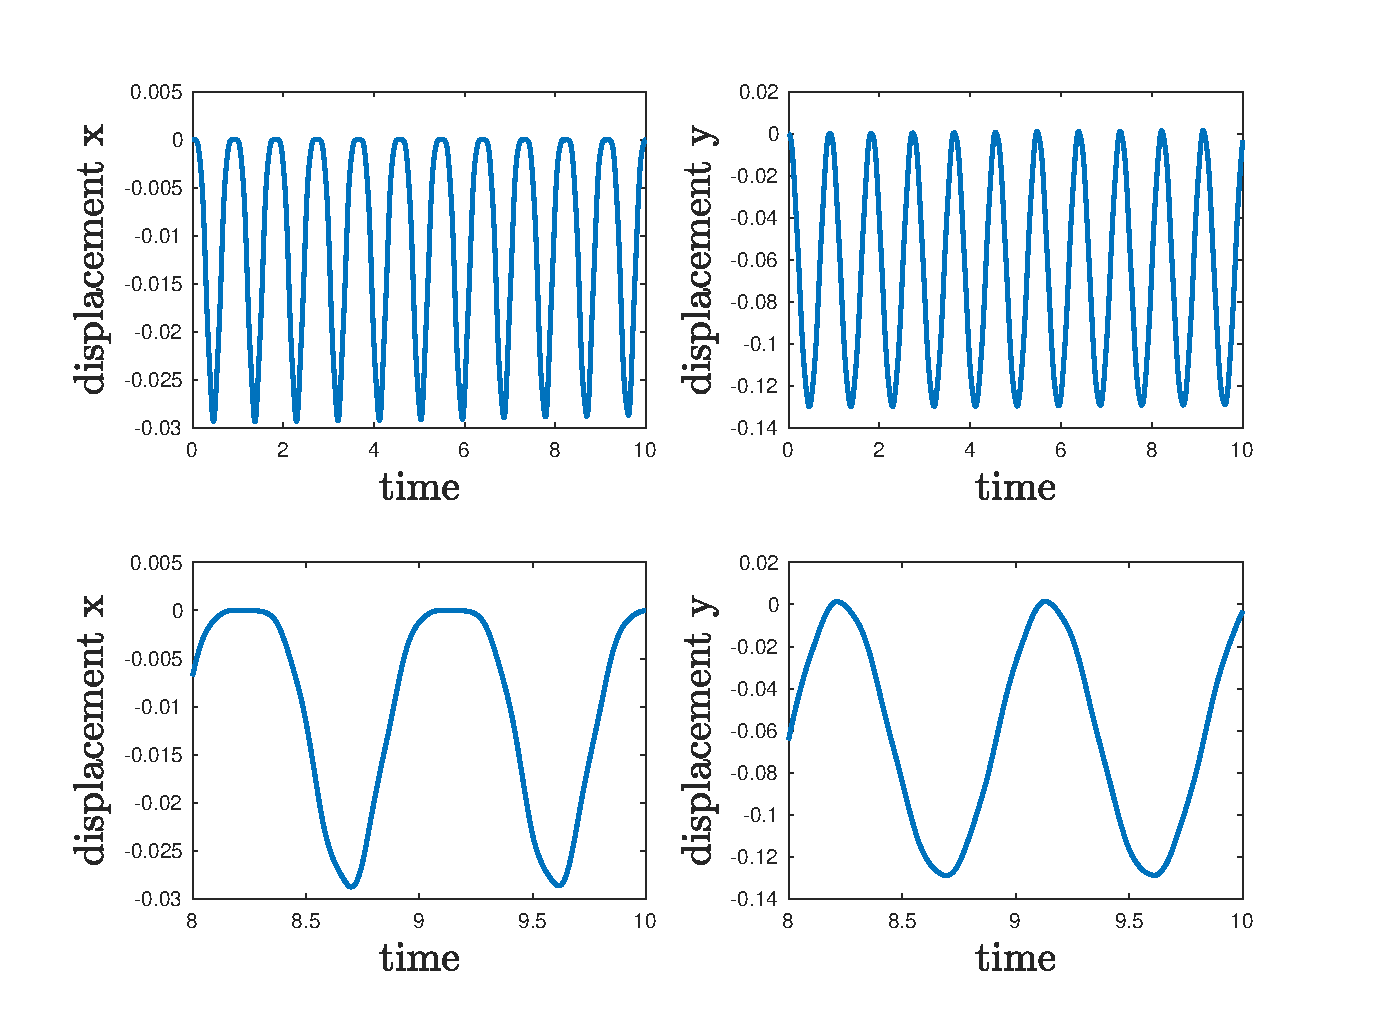
\includegraphics[width=0.8\textwidth]{CSM_2}
	%\caption{Simulated displacement of point A}
	\label{fig:CSM_2}
\end{figure}

\end{frame}

\begin{frame}
\frametitle{Structure Solver Validation}
Results for dynamic test case with time steps $dt = 0.02$, $0.01$, $0.005$
\begin{columns}
\begin{column}{0.5\textwidth}
    \begin{center}
     \includegraphics[width=0.9\textwidth]{CSM_3_data}      
     \end{center}
\end{column}
\begin{column}{0.5\textwidth}
   % \begin{center}
    % \includegraphics[width=0.9\textwidth]{fig_ldc4}      
     %\end{center}
     \begin{center}
     \includegraphics[width=0.9\textwidth]{CSM_3_sim}      
     \end{center}

\end{column}
\end{columns}

Slight differences, but closer than other references I have found \footnote{\tiny \textit{http://www.feelpp.org/benchmarks/csm/toolbox/bm-1/}}.
%https://books.google.com/books?id=-6NSKaCcGXkC&pg=PA287&lpg=PA287&dq=csm+benchmark&source=bl&ots=IOJKIrdarN&sig=PIRQDamwsj7Fs_yRQfB_pbwMWTM&hl=en&sa=X&ved=0ahUKEwjIuKDo77zZAhVJ_4MKHVU5BvI4ChDoAQhBMAU#v=onepage&q=csm%20benchmark&f=false
\end{frame}

% mesh solver? 
\section{FSI Approach}
\begin{frame}
\frametitle{FSI Approach}
Three sub-problems comprised of the fluid, structure and mesh. Structure and mesh solved in undeformed reference domains, and fluid solved in deformed domain: 

\begin{itemize}
\item Reference domain $\Omega = \Omega_F \cup \Omega_S$, $\Omega_F \cap \Omega_S = 0$
\item Deformed domain $\omega(t) = \omega_F(t) \cup \omega_S(t)$, $\omega_F(t) \cap \omega_S(t) = 0$
\item FSI interface $\Gamma_{FSI}$ (reference), $\gamma_{FSI}(t)$ (deformed) 
\end{itemize}

\end{frame}

\begin{frame}
\frametitle{FSI Approach}
The mesh is constructed in GMSH. The structure and fluid meshes are constructed separately with coincident nodes on the shared boundary. 


\FloatBarrier
\begin{figure}[h]
\centering
	\includegraphics[width=0.8\textwidth]{mesh_fluid}
	%\caption{Course mesh of fluid domain}
	\label{fig:mesh_fluid}
\end{figure}
\FloatBarrier

\FloatBarrier
\begin{figure}[h]
\centering
	\includegraphics[width=0.8\textwidth]{mesh_structure}
	\caption{Course mesh of reference structure and fluid domains}
	\label{fig:mesh_structure}
\end{figure}
\FloatBarrier



\end{frame}
\begin{frame}
\frametitle{FSI Algorithm}

\begin{enumerate}
\item Solve the fluid problem in the current fluid domain $\omega_F(t)$ 
\item Solve structure problem in reference structure domain $\Omega_s$
\item Solve mesh problem in reference fluid domain $\Omega_F$
\item Repeat steps 1-3 until convergence
\item Move to the subsequent time step
\end{enumerate} 

\end{frame}

\begin{frame}
\frametitle{Interface Traction}
Equal and opposite traction forces on interaction boundary. Cauchy stress tensor computed in current domain: 

\begin{equation}
\sigma_F = -p I + \mu_f (grad(u_f) + grad(u_f)^T )
\end{equation}

where $p$ is the fluid pressure, $\mu_f$ the dynamic viscosity and $u_f$ the fluid velocity. The fluid traction is transferred to the structure via the Piola map
\begin{equation}
 (j \sigma_F \cdot f^{-T}) \cdot n_f = -\sigma_s \cdot n_s 
\end{equation}

where $j = det (f)$ is the determinant of the Jacobi matrix $f$ computed from the mesh deformation. 

%In practice in the FSI problem, the nodal values of $\sigma_F$ are first copied to s $sigma$ defined on the reference fluid mesh. Equation this one is then computed using the fluid mesh deformation, and the reference fluid mesh and structure mesh normals. 

%Kinematic continuity 

%Want velocity of fluid to match velocity of structure on interface. Done with approximation... That's basically it. 

\end{frame}

\begin{frame}
\frametitle{Interface Traction}

\begin{itemize}
\item Fluid stress computed in current fluid domain $\omega_F(t)$
\item Fluid traction assembled in reference fluid domain $\Omega_F$ on a Continuous Galerkin degree 1 vector space 
\item Fluid traction written to an expression and applied to FSI interface $\Gamma_{FSI}$ in structure variational form 
\end{itemize}

% I want to say that fluid pressure and velocity are first stepped back from current fluid domain onto reference domain. 
%Fluid stress is calculated, and subjected to piola transform to obtain stress in reference domain. 
%Traction assembled in reference fluid domain on CG degree 1. (is degree 1 okay?) 

\end{frame}


\begin{frame}
\frametitle{Interface Velocity and Mesh Coordinates}

\begin{itemize}
\item Mesh displacement interface Dirichlet BC prescribed as structure displacement on $\Gamma_{FSI}$
\item Mesh velocity computed from current and previous time step
\item Mesh velocity interpolated to function defined on $\Gamma_{FSI}$
\item Velocity values copied to a function defined on current interface $\gamma_{FSI}$
\item Current interface velocity written to an expression and applied to $\gamma_{FSI}$ as fluid velocity Dirichlet BC
\item Fluid mesh and fluid interface mesh coordinates updated as reference coordinates plus current mesh deformation solution 
\end{itemize}
\end{frame}


%% example/sample code: 
%\begin{frame}[fragile]
% \begin{lstlisting}
%       self.u_vel.vector()[:] = (1.0/self.k)*(self.u12.vector().get_local() - self.u02.vector().get_local())
% \end{lstlisting}
%\end{frame}


\section{FSI Results}
\begin{frame}
\frametitle{FSI Results}

Printing 2-norm at each iteration of each time step asserts that: 
\begin{itemize}
\item mesh, fluid and structure velocities match on interface
\item mesh and structure displacements match on interface
\item the 2-norm of the mesh and fluid velocities reduces over iterations within a time step, as expected
\end{itemize}

A time step of $dt = 0.001$  yields physical fluid velocity and pressure results. The structure velocity behaves erratically throughout, often changing sign between time steps. Despite this the resulting structure displacement does seem reasonable until divergence after several hundred time steps. $dt = 0.0005$ yields similar results. 

Code runs without issue when bar stiffness is very high. 

\end{frame}

\begin{frame}
\frametitle{FSI Results}
\begin{figure}[h]
\centering
	\includegraphics[width=\textwidth]{t_500}
	\caption{ $dt = 0.001$, $t = 0.5s$}
	\label{fig:t_500}
\end{figure}
\end{frame}

\begin{frame}
\frametitle{FSI Results}
\begin{figure}[h]
\centering
	\includegraphics[width=\textwidth]{t_600}
	\caption{ $dt = 0.001$, $t = 0.6s$}
	\label{fig:t_600}
\end{figure}
\end{frame}

\begin{frame}
\frametitle{FSI Results}
\begin{figure}[h]
\centering
	\includegraphics[width=\textwidth]{t_700}
	\caption{ $dt = 0.001$, $t = 0.7s$}
	\label{fig:t_700}
\end{figure}
\end{frame}

\begin{frame}
\frametitle{FSI Results}
\begin{figure}[h]
\centering
	\includegraphics[width=\textwidth]{t_800}
	\caption{ $dt = 0.001$, $t = 0.8s$}
	\label{fig:t_800}
\end{figure}
\end{frame}

\begin{frame}
\frametitle{FSI Results}
\begin{figure}[h]
\centering
	\includegraphics[width=\textwidth]{t_830}
	\caption{ $dt = 0.001$, $t = 0.83s$}
	\label{fig:t_830}
\end{figure}
\end{frame}
%problem formulation and the discretization scheme
%clearly describe the problem setup, discretization method/implementation, and the coupling approach in as much detail as possible
%\end{frame}

%\begin{frame}[allowframebreaks]
%\frametitle{References }

%\bibliography{validation}{}
%\bibliographystyle{plain}
%\end{frame}
\end{document}